El verificador está compuesto por cuatro módulos, destacando principalmente los módulos
 \textit{LTL} y \textit{CTL} que implementan las interpretaciones  de las respectivas
 lógicas.
Esto permite agregar nuevos lenguajes para expresar propiedades, como pueden ser otros tipos
 de lógicas, mediante la implementación de su respectivo módulo.

En el caso de LTL se tuvo que implementar el módulo auxiliar \textit{Autómatas de Büchi}
 para manipular dichos autómatas, ya que son necesarios para el algoritmo de verificación
 de esta lógica.
Si bien este es un módulo auxiliar para la verificación de propiedades en LTL también
 es posible expresar propiedades directamente mediante estos autómatas para luego ser
 verificadas.

También se tiene un módulo destinado a los sistemas de transiciones para representar los
 modelos de los sistemas reactivos.

En la figura \ref{fig:paquetes} se muestra la integración entre los distintos módulos.

\begin{figure}[hbtp]
\begin{center}
\caption{Módulos del sistema}
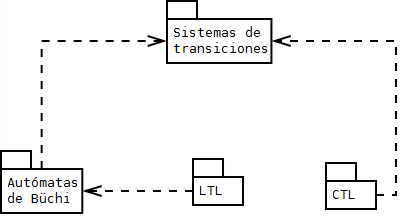
\includegraphics[width=0.7\textwidth]{mc/imagenes/paquetes.png}
\label{fig:paquetes}
\end{center}
\end{figure}


\subsection{Sistemas de transiciones}
El módulo \textit{Sistemas de transiciones} contiene la implementación de la estructura
 de un sistema de transiciones.
También se encuentran implementadas las operaciones básicas entre sistemas. De esta forma
 es posible crear sistemas de transiciones complejos a partir de sistemas más simples.
Además estas operaciones permiten modelar sistemas reactivos que interactúan entre sí.

Este módulo se compone de tres clases.
La clase principal del módulo es \texttt{TS}, que contiene la estructura y las operaciones
 necesarias para representar los sistemas de transiciones.
Además se tienen las clases \texttt{TSEstado} y \texttt{TSTransicion} para representar
 los estados y las transiciones del sistema respectivamente.

\begin{figure}[hbtp]
\begin{center}
\caption{Módulo de Sistemas de transiciones}
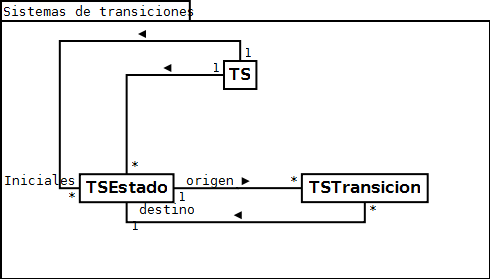
\includegraphics[width=0.8\textwidth]{mc/imagenes/ts.png}
\label{fig:modulo_TS}
\end{center}
\end{figure}

\subsubsection{Operaciones entre sistemas de transiciones}
Este módulo implementa dos de las operaciones principales entre sistemas de
 transiciones.
Las operaciones implementadas fueron vistas anteriormente y son el Intercalado y el
 \textit{Handshaking}.
Estas operaciones se encuentran implementadas en las funciones \texttt{intercaladoTS}
 y \texttt{productoSynTS} de la clase \texttt{TS}.

El autómata devuelto como resultado de cada una de estas operaciones corresponde únicamente
 a la parte alcanzable del mismo.

\subsection{Autómatas de Büchi}	
Este módulo fue implementado debido a la necesidad de tratar estos autómatas para la
 verificación de propiedades expresadas en lenguajes lineales, como LTL.

Como ya se vio en los capítulos anteriores el algoritmo de verificación para propiedades en
 LTL se basa en la construcción de un \textit{Autómata de Büchi}.
El primer paso de dicho algoritmo es traducir la propiedad a un autómata equivalente.

También es posible expresar propiedades directamente sobre estos autómatas.
Se pueden expresar las ejecuciones no deseadas con un autómata de Büchi y verificar
 si el sistema permite alguna de estas ejecuciones.
En definitiva es esto lo que realiza el algoritmo de verificación para LTL, por lo que
 esto es equivalente a saltear el primer paso del mismo.

Este módulo consta de dos clases principales.
\begin{itemize}
\item \texttt{GNBA}

Esta clase contiene la estructura los autómatas de Büchi.
Con este fin también fue necesario implementar la clase \texttt{Nodo} para representar los
 nodos de estos autómatas.

\item \texttt{ProductoTSNBA}

Esta clase contiene la información del producto entre un sistema de transiciones y un
 autómata de Büchi.

Este producto se implementó en una calse específica, ya que para generarse necesita un
 algoritmo específico. Además es la clase que implementa la parte principal del algoritmo
 de verificación.

Esta clase también puede ser parte del módulo \textit{LTL} pero finalmente se optó por
 mantenerla en este módulo ya que como se mencionó anteriormente las propiedades pueden
 ser expresadas directamente mediante autómatas y el algoritmo de verificación es el mismo.

También se implementaron las clases \texttt{ProductoTSNBANodo} y\\
 \texttt{ProductoTSNBATransicion}
 para representar los nodos y transiciones del producto respectivamente.

\end{itemize}

\begin{figure}[hbtp]
\begin{center}
\caption{Módulo de Autómatas de Büchi}
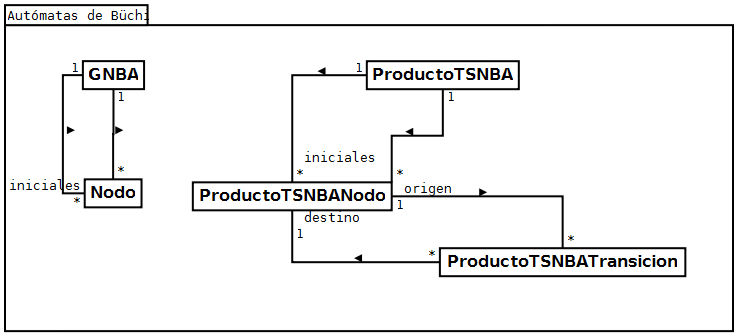
\includegraphics[width=\textwidth]{mc/imagenes/buchi.png}
\label{fig:modulo_buchi}
\end{center}
\end{figure}

\subsubsection{Construcción del producto entre un sistema de transiciones y un autómata de Büchi}
Este producto genera como resultado un nuevo autómata, el cuál está representado
 por la clase \texttt{ProductoTSNBA}.

Esta clase implementa el algoritmo de contrucción de este producto mediante
 la función \texttt{ProductoTSNBA(ts, nba)}, donde:
\begin{itemize}
\item \texttt{ts} es un sistema de transiciones.
\item \texttt{nba} es un autómata de Büchi.
\end{itemize}

Esta función devuelve la parte alcanzable del producto.

\subsubsection{Verificación de propiedadades}
Una vez obtenido el producto mencionado en la sección anterior el siguiente paso
 es verificar si existen palabras reconocidas por este autómata.

Como se vio en capítulos anteriores, como el autómata reconoce las palabras que no cumplen
 la propiedad deseada, este proceso es equivalente encontrar las ejecuciones del sistema
 que no cumplen la propiedad.
En caso de existir al menos una, esta es un contrajemplo que muestra que el sistema no
 cumple dicha propiedad.

Este proceso se encuentra implementado en la función \texttt{verificar()} de la clase
 \texttt{ProductoTSNBA}.
Esta función se basa en el recorrido DFS para buscar un ciclo en el autómata.
Este ciclo debe pasar por al menos un estado de cada conjunto de aceptación del
 autómata, como se vio en el capítulo correspondiente a Autómatas de Büchi.

\subsection{LTL}
El módulo \textit{LTL} está comprendido por las clases necesarias para implementar dicha
 lógica.
En la figura \ref{fig:modulo_LTL} se muestran las relaciones entre la clase \texttt{FormulaLTL}
 y todas sus especializaciones que implementan la sintaxis y semántica de LTL.

\begin{figure}[hbtp]
\begin{center}
\caption{Módulo de LTL}
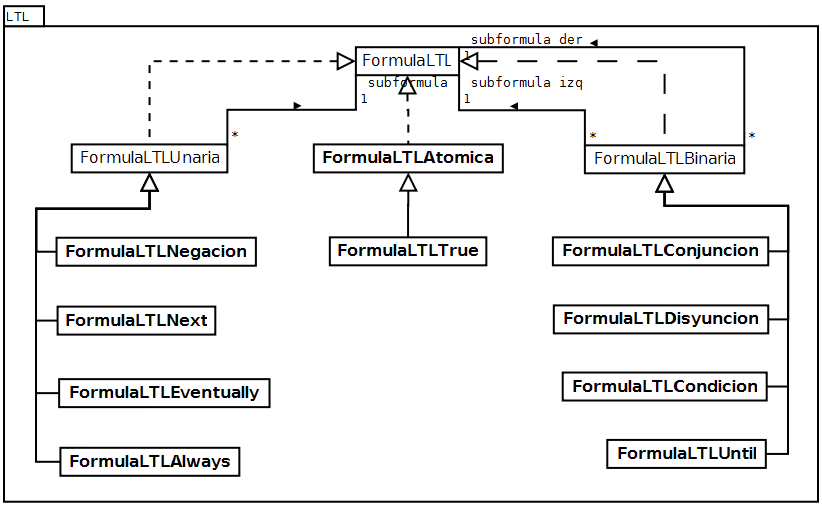
\includegraphics[width=\textwidth]{mc/imagenes/ltl.png}
\label{fig:modulo_LTL}
\end{center}
\end{figure}

Es importante destacar que este módulo no implementa el algoritmo de verificación para LTL.
El algoritmo es implementado en su mayor parte por el módulo \textit{Autómatas de Büchi}.
El módulo \textit{LTL} simplemente traduce la fórmula a verificar en un autómata equivalente
 y traslada la responsabilidad de la verificación al módulo correspondiente.

La clase que inicia el proceso de verificación es \texttt{LTLMC}.
El único objetivo de esta clase es implementar la función \texttt{verificar(ts, formula)},
 donde:
\begin{itemize}
\item \texttt{ts} es un sistema de transiciones.
\item \texttt{formula} es una fórmula LTL.
\end{itemize}

Esta función es la encargada de iniciar el proceso de verificación traduciendo la fórmula LTL
 al autómata correspondiente, delegar la verificación al módulo de \textit{Autómatas de Büchi}
 y luego desplegar el resultado de la misma.

\subsection{CTL}
Este módulo al igual que el módulo anterior implementa la sintaxis y semántica de CTL.
Pero a diferencia del módulo \textit{LTL} este implementa el algoritmo de verificación.
Esto se debe a que el algoritmo para este tipo de lógica no requiere la implementación
 de módulos ni estructuras auxiliares.
Este algoritmo se basa en el cálculo del conjunto de satisfacibilidad de una fórmula
 y sus subfórmulas. Se encuentra implementado en la función \texttt{verificar(ts, formula)},
 donde:
\begin{itemize}
\item \texttt{ts} es un sistema de transiciones.
\item \texttt{formula} es una fórmula CTL.
\end{itemize}

Esta función verifica que el conjunto de los estados iniciales de \texttt{ts} esté
 incluído en el conjunto de satisfacibilidad de \texttt{formula}, tal como se vio
 en el capítulo de CTL.
Además esta función se encuentra en la clase \texttt{CTLMC}, cuyo único objetivo es
 alojar la misma.

Por otro lado el cálculo del conjunto de satisfacibilidad se encuentra definido en la
 función \texttt{getSat(ts)} de la clase \texttt{FormulaCTL}, donde \texttt{ts} es un
 sistema de transiciones.

\begin{figure}[hbtp]
\begin{center}
\caption{Módulo de CTL}
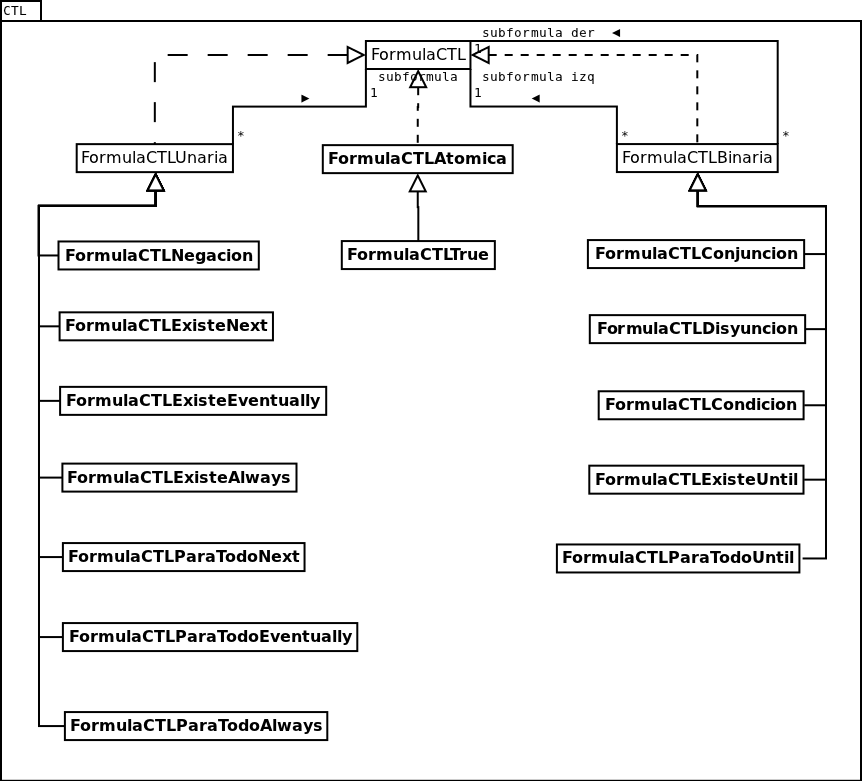
\includegraphics[width=\textwidth]{mc/imagenes/ctl.png}
\label{fig:modulo_CTL}
\end{center}
\end{figure}
